\documentclass[10pt]{article}
\usepackage[margin=0.75in]{geometry}
\usepackage[T1]{fontenc}
\usepackage{lmodern,microtype,booktabs,longtable,array,graphicx,amsmath}
\usepackage[hidelinks]{hyperref}
\hypersetup{pdftitle={Offline Training and Online Inference for a Tiny Stride Prefetcher}}
\setlength{\parindent}{0pt}
\setlength{\parskip}{5pt}
\setlength{\tabcolsep}{4pt}
\title{Offline Training and Online Inference\\\large A Tiny Neural Stride Prefetcher on 602.gcc\_s-734B}
\author{602 Stride dynamic inference experiment}
\date{Measured ChampSim execution; frozen deployment scope}
\begin{document}
\maketitle
\section{Direct answer: one new access, carried history, measured advantage}

Each prediction consumes \textbf{one new eligible L2 LOAD access}. Its PC and aligned byte address become a tensor of shape $(1,1,128)$. History is carried through the exact PC's continuous LSTM h/c, each of shape $(1,1,H)$. There is no multi-access warm-up requirement or last-W recomputation. Runtime weights remain fixed. The 128 features, H hidden values and K output addresses are not instruction or access counts.

In the cold slice, h16-i20m first has all three cumulative quality metrics strictly above matched Stride at the recorded point $N=2,600,000$ retired instructions and $D=41,990$ completed L2 decisions. Coverage / selected accuracy / legacy timeliness are 58.108\% / 31.354\% / 100.000\%, versus Stride's 17.216\% / 29.762\% / 99.973\%.

The consecutive recorded cumulative advantage lasts through $N=18,000,000$ and $D=291,480$; the first recorded exit is $N=18,100,000$ because accuracy falls below Stride. At entry, IPC is 0.406830, cumulative saving is 759,702 cycles, request pressure is 0.945 and L2 occupancy is 4,096/4,096 lines.

In the separate summer-compatible protocol, h8-i1m first strictly exceeds BOTH references at $N=20,500,000$, $D=331,714$. Coverage / accuracy / timeliness are 57.777\% / 28.672\% / 99.973\%; Stride: 17.116\% / 28.632\% / 99.440\%; original summer h8-i20m: 57.376\% / 27.372\% / 99.904\%. The recorded cumulative advantage persists through $N=25,000,003$, $D=404,219$ (4,500,003 further instructions). This is quality superiority: its final execution still takes 15,757 more cycles than summer.

With the retained 4/16-MAC inference costs, h8-i1m has no strict three-quality joint win over Stride; end-to-end losses are 460,332 / 391,755 cycles. High timeliness accompanies only 0.258\% / 0.643\% useful coverage. Queueing, dropped work and redundant requests remain visible.

N denotes retired instructions since the evaluation boundary. Historical total simulated retirement is N+25,000,004 (45,500,004 at joint entry); cold total retirement is N because skipped records are not simulated. These descriptive points are not minimum-history requirements. At the cold entry point the NN has 39,679 issued requests (12,441 useful); the distinction is not based on a handful of requests. The preceding point ties in timeliness. No new stability threshold or policy change is introduced.

\clearpage\section{What a prediction actually observes}

\begin{center}\scriptsize
\begin{tabular}{ll}
\toprule
Quantity & Actual forward meaning \\
\midrule
New inputs & 1 L2 LOAD; PC and aligned 64-byte address \\
Encoded tensor & $(1,1,128)$ FP32 bits: 64 PC + 64 address \\
Projected input & $(1,1,H)$ after the existing tanh projection \\
Carried h/c & $(1,1,H)$ each; exact-PC state lifetime \\
Output & Learned silent/act, learned positive K, free-running signed deltas \\
\bottomrule
\end{tabular}\end{center}

At service start the engine selects the last completed h/c for this PC. On a successful completion it installs the new h/c and increments that state lifetime's observed update count. A different PC selects a different entry. Eviction starts a new lifetime at zero. Queued, dropped and unfinished events are not completed state updates. Silent decisions still update h/c. The decoder's temporary recurrent state is separate from the carried encoder history.

Retired N labels execution progress. Eligible, admitted, started and completed D count actual callbacks/service events; out-of-order observation can precede retirement. The trace reader's look-ahead is never counted as predictor input. Offline i1m/i20m are pretraining budgets, separate from all runtime counts.

Having updated h/c k times describes its history of use. It neither means the model remembers k accesses in full nor proves k accesses are sufficient. Measurement snapshots leave h/c and the output policy unchanged.

\subsection{A real interleaved-PC sequence}

\begin{center}\scriptsize
\begin{tabular}{rllrrr}
\toprule
Decision & PC & Line & Life & Prior / post updates & act/K \\
\midrule
12 & 4257639 & 702,778,647,070 & 12 & 0 to 1 & 0/0 \\
13 & 4257930 & 702,778,646,955 & 13 & 0 to 1 & 0/0 \\
14 & 4257008 & 702,778,646,867 & 14 & 0 to 1 & 1/1 \\
15 & 4257721 & 702,778,647,038 & 15 & 0 to 1 & 1/1 \\
16 & 4257076 & 702,778,646,957 & 2 & 1 to 2 & 0/0 \\
17 & 4257546 & 702,778,647,039 & 16 & 0 to 1 & 0/0 \\
18 & 4257551 & 702,778,646,958 & 17 & 0 to 1 & 0/0 \\
19 & 4257721 & 702,778,647,104 & 15 & 1 to 2 & 1/1 \\
\bottomrule
\end{tabular}\end{center}

These are consecutive completed events from the actual frozen h8-i1m run. Full old/new h/c vectors, timestamps, N/D and candidate addresses are retained in history\_example.csv. The table indexes the old state by PC and lifetime; it does not substitute a synthetic access sequence.

On the repeated PC 4257721 at N=284, h[0] changes from 0.217924 to 0.462595, and c[0] from 0.254614 to 0.566886. These are components of the actual carried vectors, whose full contents are in the CSV. Line values above are multiplied by 64 to form the aligned byte-address feature.

\clearpage\section{Strict three-quality comparison rules}

Each comparison uses one NN run and one fixed reference run at the exact same recorded N or interval $(N_a,N_b]$. Coverage is U/M0, selected accuracy is U/(Ipf-Q), and legacy timeliness is U/(U+L). Raw U/Ipf is also retained. All three differences must be strictly positive; exact integer fractions distinguish equality from strict superiority. Ties are NONLOWER\_WITH\_TIE, undefined denominators are NA, and missing or unaligned references are separate from measured non-attainment.

The original summer reference is the compact hurdle v9 seed-7 i20m model of the same hidden size. Its checkpoint bytes, action stream and 30 end metrics match the prefix-sweep i20m artifacts. New measurements replay that original stream with the unchanged keyed ListReplayer. Separate offline\_same\_checkpoint comparisons retain each i1m/i20m point's own original replay, rather than selecting the best budget after seeing results.

Historical comparisons use 25M no-prefetch warmup, empty predictor state at measurement start, and the original 25M measurement (actual origin 25,000,004; final N 25,000,003). The newly measured conventional Stride is also gated throughout warmup. Its original offline Stride replay is retained separately. Cold starts use a fresh cache at the skipped 25M boundary; there is no compatible cold summer reference and no cross-protocol joint assertion.

\subsection{Cold cumulative outcomes}

\begin{center}\scriptsize
\begin{tabular}{llrrr}
\toprule
NN & Reference & First recorded N / completed D & Points & Intervals \\
\midrule
h16-i1m & stride & Not reached & 0 & 0 \\
h8-i1m & stride & Not reached & 0 & 0 \\
h16-i20m & stride & 2,600,000 / 41,990 & 155 & 1 \\
h8-i20m & stride & Not reached & 0 & 0 \\
\bottomrule
\end{tabular}\end{center}

\subsection{Summer-compatible cumulative outcomes}

\begin{center}\scriptsize
\begin{tabular}{llrrr}
\toprule
NN & Reference & First recorded N / completed D & Points & Intervals \\
\midrule
h16-i1m & stride & Not reached & 0 & 0 \\
h8-i1m & stride & 20,500,000 / 331,714 & 47 & 1 \\
h16-i20m & stride & Not reached & 0 & 0 \\
h8-i20m & stride & Not reached & 0 & 0 \\
h16-i1m & summer & Not reached & 0 & 0 \\
h8-i1m & summer & 18,300,000 / 296,254 & 69 & 1 \\
h16-i20m & summer & Not reached & 0 & 0 \\
h8-i20m & summer & Not reached & 0 & 0 \\
h16-i1m & stride\_and\_summer & Not reached & 0 & 0 \\
h8-i1m & stride\_and\_summer & 20,500,000 / 331,714 & 47 & 1 \\
h16-i20m & stride\_and\_summer & Not reached & 0 & 0 \\
h8-i20m & stride\_and\_summer & Not reached & 0 & 0 \\
h16-i1m & offline\_same\_checkpoint & Not reached & 0 & 0 \\
h8-i1m & offline\_same\_checkpoint & Not reached & 0 & 0 \\
h16-i20m & offline\_same\_checkpoint & Not reached & 0 & 0 \\
h8-i20m & offline\_same\_checkpoint & Not reached & 0 & 0 \\
\bottomrule
\end{tabular}\end{center}

\clearpage\section{Where each advantage begins and ends}

The following lists every maximal strictly exceeding segment at the retained scales. For cumulative rows the endpoints are recorded points, not claims about unsampled instants. For interval rows $(a,b]$ is the union of consecutive satisfying counter windows. The exit column gives the first subsequent failing/tied/undefined observation. The full status segments, raw denominators, separate metric differences and exits are in quality\_intervals.csv and quality\_points.csv.

\subsection{Cold versus Stride}

\scriptsize\begin{longtable}{lllrr}\toprule NN & Reference & Scale & Range N & First exit N \\\midrule\endhead
h16-i1m & stride & 100k & 11,800,000--11,900,000 & 12,000,000 \\
h16-i20m & stride & cumulative & 2,600,000--18,000,000 & 18,100,000 \\
h16-i20m & stride & 100k & 4,800,000--5,000,000 & 5,100,000 \\
h16-i20m & stride & 100k & 5,700,000--5,800,000 & 5,900,000 \\
h16-i20m & stride & 100k & 6,400,000--6,500,000 & 6,600,000 \\
h16-i20m & stride & 100k & 7,800,000--7,900,000 & 8,000,000 \\
h16-i20m & stride & 100k & 8,500,000--8,800,000 & 8,900,000 \\
h16-i20m & stride & 100k & 8,900,000--9,000,000 & 9,100,000 \\
h16-i20m & stride & 100k & 9,100,000--9,200,000 & 9,300,000 \\
h16-i20m & stride & 100k & 9,600,000--9,700,000 & 9,800,000 \\
h16-i20m & stride & 100k & 11,400,000--11,500,000 & 11,600,000 \\
h16-i20m & stride & 100k & 11,800,000--11,900,000 & 12,000,000 \\
h16-i20m & stride & 100k & 12,400,000--12,500,000 & 12,600,000 \\
h16-i20m & stride & 100k & 12,700,000--12,800,000 & 12,900,000 \\
h16-i20m & stride & 1m & 2,000,000--3,000,000 & 4,000,000 \\
h16-i20m & stride & 1m & 4,000,000--10,000,000 & 11,000,000 \\
h16-i20m & stride & 1m & 11,000,000--13,000,000 & 14,000,000 \\
h8-i20m & stride & 100k & 7,800,000--7,900,000 & 8,000,000 \\
h8-i20m & stride & 100k & 9,100,000--9,200,000 & 9,300,000 \\
h8-i20m & stride & 100k & 11,800,000--11,900,000 & 12,000,000 \\
h8-i20m & stride & 100k & 23,300,000--23,400,000 & 23,500,000 \\\bottomrule\end{longtable}\normalsize

\subsection{Summer-compatible references}

\scriptsize\begin{longtable}{lllrr}\toprule NN & Reference & Scale & Range N & First exit N \\\midrule\endhead
h8-i1m & stride & cumulative & 20,500,000--25,000,003 & NA \\
h8-i1m & summer & cumulative & 18,300,000--25,000,003 & NA \\
h8-i1m & stride\_and\_summer & cumulative & 20,500,000--25,000,003 & NA \\
h8-i1m & stride & 100k & 13,800,000--13,900,000 & 14,000,000 \\
h8-i1m & stride & 100k & 15,300,000--15,400,000 & 15,500,000 \\
h8-i1m & stride & 100k & 15,900,000--16,000,000 & 16,100,000 \\
h8-i1m & stride & 100k & 16,500,000--16,600,000 & 16,700,000 \\
h8-i1m & stride & 100k & 17,200,000--17,300,000 & 17,400,000 \\
h8-i1m & stride & 100k & 17,600,000--17,700,000 & 17,800,000 \\
h8-i1m & stride & 100k & 20,100,000--20,300,000 & 20,400,000 \\
h8-i1m & stride & 100k & 22,600,000--22,700,000 & 22,800,000 \\
h8-i1m & stride & 100k & 22,800,000--22,900,000 & 23,000,000 \\
h8-i1m & stride & 100k & 24,100,000--24,200,000 & 24,300,000 \\
h8-i1m & summer & 100k & 19,500,000--19,600,000 & 19,700,000 \\
h8-i1m & stride & 1m & 13,000,000--14,000,000 & 15,000,000 \\
h8-i1m & stride & 1m & 15,000,000--18,000,000 & 19,000,000 \\
h8-i1m & stride & 1m & 20,000,000--21,000,000 & 22,000,000 \\
h8-i1m & stride & 1m & 22,000,000--23,000,000 & 24,000,000 \\
h8-i1m & stride & 1m & 24,000,000--25,000,000 & NA \\
h8-i1m & summer & 1m & 19,000,000--20,000,000 & 21,000,000 \\
h8-i1m & summer & 1m & 24,000,000--25,000,000 & NA \\
h8-i1m & stride\_and\_summer & 1m & 24,000,000--25,000,000 & NA \\
h16-i20m & stride & 100k & 13,800,000--13,900,000 & 14,000,000 \\
h16-i20m & stride & 100k & 15,300,000--15,400,000 & 15,500,000 \\
h16-i20m & stride & 100k & 15,900,000--16,000,000 & 16,100,000 \\
h16-i20m & stride & 100k & 16,500,000--16,600,000 & 16,700,000 \\
h16-i20m & stride & 100k & 17,200,000--17,300,000 & 17,400,000 \\
h16-i20m & stride & 100k & 17,600,000--17,700,000 & 17,800,000 \\
h16-i20m & stride & 100k & 20,100,000--20,300,000 & 20,400,000 \\
h16-i20m & stride & 100k & 22,600,000--22,700,000 & 22,800,000 \\
h16-i20m & stride & 100k & 22,800,000--22,900,000 & 23,000,000 \\
h16-i20m & stride & 100k & 24,100,000--24,200,000 & 24,300,000 \\
h16-i20m & stride & 1m & 15,000,000--18,000,000 & 19,000,000 \\
h16-i20m & stride & 1m & 20,000,000--21,000,000 & 22,000,000 \\
h16-i20m & stride & 1m & 22,000,000--23,000,000 & 24,000,000 \\
h16-i20m & stride & 1m & 24,000,000--25,000,000 & NA \\
h8-i20m & stride & 100k & 9,100,000--9,200,000 & 9,300,000 \\
h8-i20m & stride & 100k & 15,900,000--16,000,000 & 16,100,000 \\\bottomrule\end{longtable}\normalsize

\clearpage\section{Cumulative quality differences versus Stride}

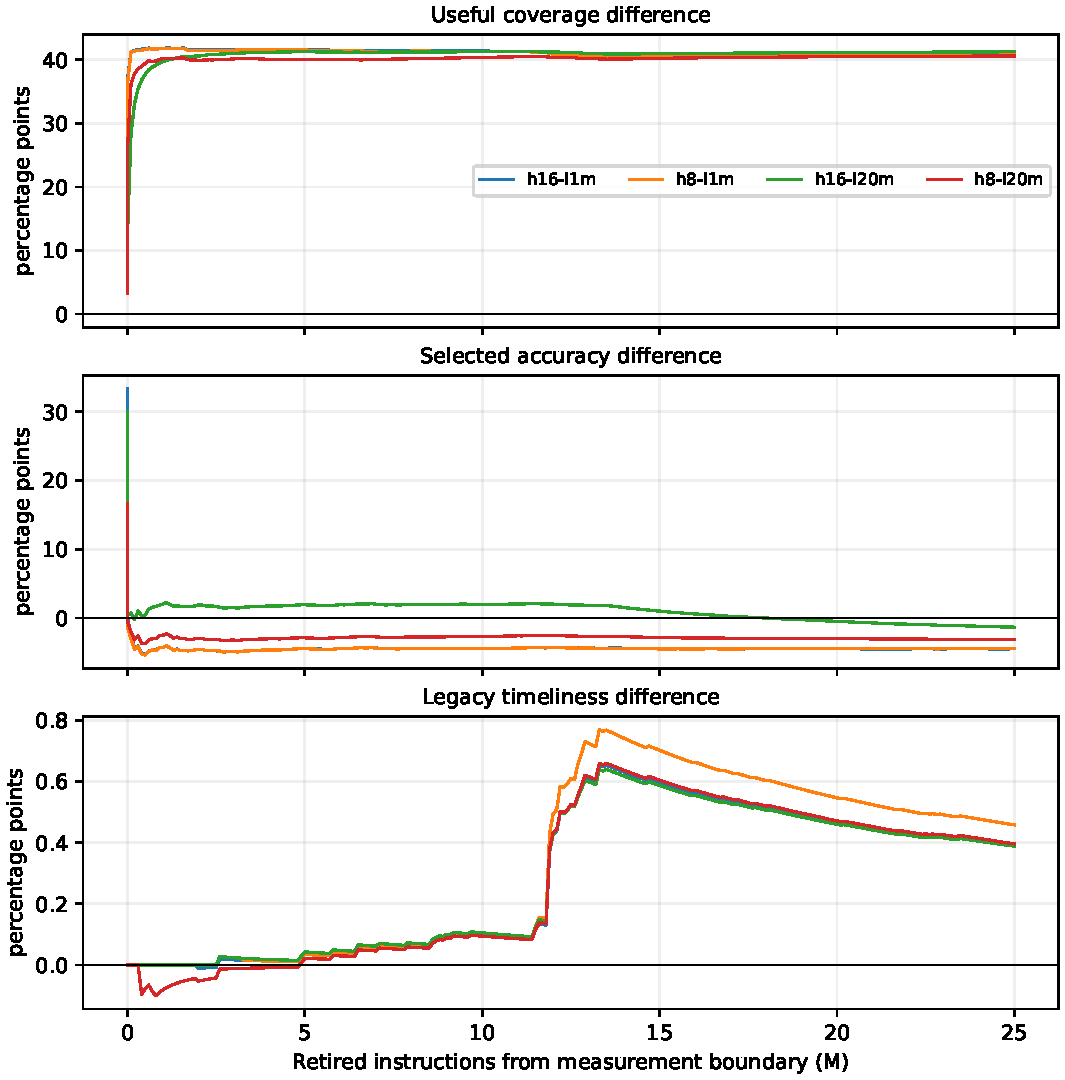
\includegraphics[width=\linewidth]{figures/strict_cold_quality.pdf}

All three differences must be above zero together. A cumulative winning interval does not mean every local window wins: h16-i20m wins 15 of 250 existing 100k windows and 9 of 25 existing 1M windows. No threshold is fitted to turn these descriptive counts into a stability guarantee.

\clearpage\section{Cumulative quality differences versus original summer}

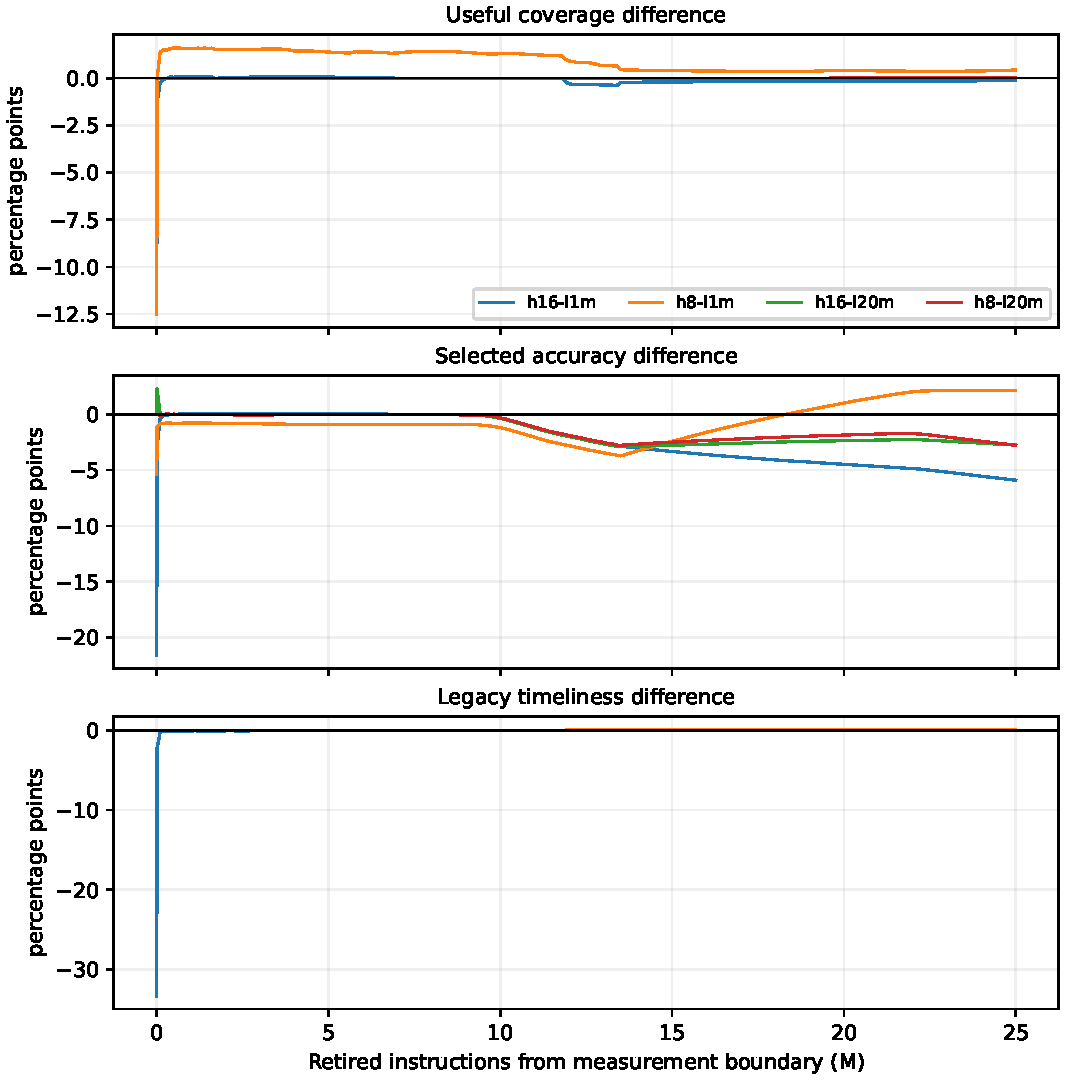
\includegraphics[width=\linewidth]{figures/strict_summer_quality.pdf}

The original summer comparison is confined to its compatible warm-cache protocol. The same-H i20m reference is fixed for every point of a live run.

\clearpage\section{Request lifecycles and actual inference delays}

Legacy interval ratios describe activity in that interval, including usefulness credited to prefetches requested earlier. They are not issue-cohort success probabilities. The existing 100k issue cohorts follow requests to run end; pending and resident-unused requests remain censored. At the cold h16-i20m entry N=2.6M, the legacy useful count is 12,441; final follow-up of those issue cohorts has 12,449 timely requests and 2 censored requests. At the entry snapshot itself, 75 resident-unused requests remain unresolved. None is declared a failure at that boundary.

\begin{center}\scriptsize
\begin{tabular}{lrrrrrrr}
\toprule
Case & Eligible & Done & Wait cycles & Arrival-to-done & Drops & Max KiB & Peak envelope \\
\midrule
cold\_history\_h8\_i1m & 404,271 & 404,271 & 0.000 & 0.000 & 0 & NA & 17.516 \\
cold\_history\_h8\_i1m\_mac16 & 404,271 & 152,062 & 7,122.134 & 7,575.153 & 252,192 & 16.414 & 15.148 \\
cold\_history\_h8\_i1m\_mac4 & 404,271 & 84,091 & 13,000.783 & 13,820.820 & 320,163 & 16.414 & 14.586 \\
\bottomrule
\end{tabular}\end{center}

\begin{center}\scriptsize
\begin{tabular}{lrrrrr}
\toprule
Case & Mean prior updates & Max prior & Zero-prior decisions & Max wait cycles & Max completion cycles \\
\midrule
cold\_history\_h8\_i1m & 44,367.94 & 118,329 & 92 & 0 & 0 \\
cold\_history\_h8\_i1m\_mac16 & 18,065.19 & 51,903 & 63 & 9,031 & 9,596 \\
cold\_history\_h8\_i1m\_mac4 & 10,148.97 & 29,055 & 57 & 15,495 & 16,466 \\
\bottomrule
\end{tabular}\end{center}

The bounded history logs retained complete early records but each has one truncated final buffered record; that tail is explicitly excluded. The selected consecutive excerpts are complete, and all final aggregate counters are complete. The logger now flushes each bounded row, validated by the regression tests. The three instrumented full runs still match all 90 original end-counter fields.

Wait means use started decisions; completed service and arrival-to-completion means use completed decisions. Endpoint queues/inference remain pending. Added lifetime counters and bounded first-1,024-event logging are measurement overhead, not predictor features or deployment SRAM. Weights, PC state, inference scratch and queues retain their full FP32 deployment accounting; offline training memory is excluded. The original finite-service negative results and cache occupancy/turnover measurements follow.

\clearpage\section{Causal inference and matched conditions}

Only the 64-bit PC and 64-bit aligned byte address enter the neural encoder. A 128-to-H projection and LSTM update h/c for the exact PC. The learned hurdle selects emission; the positive-count head determines K; a GRU decoder emits direct signed cache-line deltas with free-running predicted feedback. Conventional Stride is a separate baseline, retaining its current-line first requests [current, current + stride], tracker behavior and page restrictions. It is not a runtime neural teacher.

The serial inference engine consumes a bounded 16-event input FIFO. A decision uses the last completed h/c for its exact PC. State and outputs become visible at scheduled completion, so queued accesses cannot see a future recurrent state. A finite table has 64 exact-PC entries with LRU replacement; an unbounded control isolates capacity effects. Frozen weights need one active FP32 copy. There is no parameter publication operation.

Historical compatibility preserves the original 25M no-prefetch cache warmup plus 25M measurement, zero modeled neural cost, unbounded PC routing and empty predictor state at the measurement boundary. The actual warmup retirement group ends after 25,000,004 instructions, followed by 25,000,003 measured instructions. The old conventional live Stride run issued throughout warmup and is not used as its matched cycle-saving reference.

The primary protocol is \emph{cold start at the held-out trace-slice boundary}. It skips exactly 25,000,000 opaque records using the actual compiled reader types, without simulating them or warming caches. It executes exactly the next 25,000,000 selected instructions with fresh caches and recurrent histories, loading only pretrained weights. This is not a program-startup experiment. All methods use the same selected records and cache configuration; actual callback order/timing may differ in closed-loop live execution.

Retired target instructions from that boundary are the horizontal axis. Eligible L2 callbacks, admitted decisions and completed decisions are distinct from trace read-ahead and retirement. Snapshots at 0, 1k, 10k and every 100k retired instructions retain startup costs. Curves use exact one-million-instruction counter intervals; cumulative cycle saving always compares matched cold references.

\subsection{Assumed inference service}

The functional control has zero modeled cost. Sensitivity cases use 4 or 16 MACs/cycle with matched 16 or 64-byte/cycle weight and scratch bandwidth, one nonlinear unit taking four cycles per operation, and serialized dense/nonlinear/memory/control phases. Initiation interval equals data-dependent service time. For hidden size H and actual decoded count K, the forward work is

\[W_{MAC}=128H+8H^2+2H+eH+K(3H^2+4H),\quad W_{NL}=6H+e+K(3H+1),\]

where e is the learned emission decision. Control costs 8 + ceil(entries/4) + 4K cycles; additional scratch traffic is 4(128+4H)+24K bytes. The cold decoder resource permits 32 outputs, with excess and numerical failures counted. A 32-address output FIFO releases at most one request/cycle in finite cases through the original request path and duplicate/drop behavior. An unconditional per-core-cycle hook services pending work even when no demand callback occurs. Host execution time is never converted to CPU stall cycles. These are architectural sensitivity assumptions, not measured silicon timing, area, power or synthesized frequency.

\clearpage\section{Cold end-to-end measurements}

All rows execute 25,000,000 instructions and observe 404,271 L2 LOAD callbacks. H8/H16 i1m/i20m use the existing seed-7 pretrained weights; they do not represent independent pretraining seeds. State0 denotes the unbounded algorithmic control; state64 is finite LRU. Zero denotes zero modeled neural service cost.

\begin{center}
\scriptsize
\begin{tabular}{lrrrr}
\toprule
Method & IPC & Cycles & Saved vs Stride & L2 MPKI \\
\midrule
h16 frozen i1m & 0.406523 & 61,497,175 & 7,000,550 & 3.401 \\
h8 frozen i1m & 0.406066 & 61,566,400 & 6,931,325 & 3.419 \\
h8 frozen i1m /64 /MAC0 & 0.406064 & 61,566,690 & 6,931,035 & 3.419 \\
h8 frozen i1m /64 /MAC16 & 0.362900 & 68,889,480 & -391,755 & 8.098 \\
h8 frozen i1m /64 /MAC4 & 0.362539 & 68,958,057 & -460,332 & 8.130 \\
h16 frozen i20m & 0.406818 & 61,452,480 & 7,045,245 & 3.391 \\
h8 frozen i20m & 0.406250 & 61,538,423 & 6,959,302 & 3.444 \\
No prefetch & 0.362511 & 68,963,505 & -465,780 & 8.151 \\
Stride & 0.364976 & 68,497,725 & 0 & 6.755 \\
\bottomrule
\end{tabular}
\end{center}

\begin{center}
\scriptsize
\begin{tabular}{lrrrrrr}
\toprule
Method & Coverage & Miss reduction & Raw acc. & Selected acc. & Timeliness & P/NL \\
\midrule
h16 frozen i1m & 0.5828 & 0.5827 & 0.2436 & 0.2436 & 0.9992 & 1.2057 \\
h8 frozen i1m & 0.5805 & 0.5805 & 0.2437 & 0.2437 & 0.9998 & 1.2008 \\
h8 frozen i1m /64 /MAC0 & 0.5805 & 0.5805 & 0.2437 & 0.2437 & 0.9998 & 1.2008 \\
h8 frozen i1m /64 /MAC16 & 0.0064 & 0.0064 & 0.0079 & 0.0079 & 0.9985 & 0.4118 \\
h8 frozen i1m /64 /MAC4 & 0.0026 & 0.0026 & 0.0057 & 0.0057 & 0.9887 & 0.2272 \\
h16 frozen i20m & 0.5839 & 0.5839 & 0.2751 & 0.2751 & 0.9991 & 1.0698 \\
h8 frozen i20m & 0.5775 & 0.5774 & 0.2573 & 0.2573 & 0.9992 & 1.1314 \\
No prefetch & 0.0000 & 0.0000 & NA & NA & NA & 0.0000 \\
Stride & 0.1713 & 0.1713 & 0.2884 & 0.2884 & 0.9952 & 0.2994 \\
\bottomrule
\end{tabular}
\end{center}

\subsection{Raw counter meanings}

Let M0 be same-protocol no-prefetch L2 LOAD misses, M method misses, NL L2 LOADs, P requested prefetches, Ipf issued prefetches, Q PQ-merged requests, U useful and L late. The original parser and formulas are preserved:

\[\text{coverage}=U/M0,\quad\text{miss reduction}=(M0-M)/M0,\quad\text{raw accuracy}=U/Ipf,\]\[\text{selected accuracy}=U/(Ipf-Q),\quad\text{legacy timeliness}=U/(U+L),\quad\text{pressure}=P/NL.\]

Undefined ratios are NA. Legacy useful may include a first RFO; NL and M retain the original LOAD counter scope. Coverage is not imitation accuracy. Unused eviction and one minus accuracy are not direct cache pollution measurements.

\begin{center}
\scriptsize
\begin{tabular}{lrrrrrr}
\toprule
Method & M & P & Ipf & Q & U & L \\
\midrule
h16 frozen i1m & 85,022 & 487,444 & 487,444 & 0 & 118,744 & 99 \\
h8 frozen i1m & 85,475 & 485,458 & 485,458 & 0 & 118,291 & 25 \\
h8 frozen i1m /64 /MAC0 & 85,477 & 485,437 & 485,437 & 0 & 118,288 & 25 \\
h8 frozen i1m /64 /MAC16 & 202,455 & 166,466 & 166,466 & 0 & 1,310 & 2 \\
h8 frozen i1m /64 /MAC4 & 203,238 & 91,858 & 91,858 & 0 & 526 & 6 \\
h16 frozen i20m & 84,784 & 432,486 & 432,486 & 0 & 118,982 & 108 \\
h8 frozen i20m & 86,101 & 457,373 & 457,373 & 0 & 117,666 & 98 \\
No prefetch & 203,764 & 0 & 0 & 0 & 0 & 0 \\
Stride & 168,865 & 121,020 & 121,020 & 0 & 34,900 & 168 \\
\bottomrule
\end{tabular}
\end{center}

\clearpage\section{Recorded runtime observations}

The following h8-i1m zero-cost rows use already recorded cumulative snapshots at 100k, 1M and 25M retired instructions after the 25M trace-slice boundary. Coverage uses NoPF misses at the same recorded instruction count. They are descriptive sample points, not minimum-history requirements, optimized observation budgets or runtime triggers.

\begin{center}
\small
\begin{tabular}{rrrrr}
\toprule
Retired instructions & Eligible L2 callbacks & NN completed & Cumulative IPC & Valid L2 lines \\
\midrule
100,000 & 1,659 & 1,659 & 0.362541 & 1,419 / 4,096 \\
1,000,000 & 16,196 & 16,196 & 0.405151 & 4,096 / 4,096 \\
25,000,000 & 404,271 & 404,271 & 0.406066 & 4,096 / 4,096 \\
\bottomrule
\end{tabular}
\end{center}

\begin{center}
\small
\begin{tabular}{rrrrrr}
\toprule
Retired instructions & Coverage & Raw accuracy & Selected accuracy & Timeliness & P/NL \\
\midrule
100,000 & 0.5535 & 0.3996 & 0.3996 & 1.0000 & 1.1706 \\
1,000,000 & 0.5863 & 0.2592 & 0.2592 & 1.0000 & 1.2006 \\
25,000,000 & 0.5805 & 0.2437 & 0.2437 & 0.9998 & 1.2008 \\
\bottomrule
\end{tabular}
\end{center}

The PC's h/c is carried continuously through successive completed inference events. Snapshot collection and the plotted counter intervals do not reset, truncate or otherwise change that history. No fixed-length history window W is introduced. Weights remain unchanged. The L2 callback count is the actual observation count; at the 1M snapshot it is 16,196, while the legacy completed LOAD counter is 16,195 because callback observation and cache completion have different timing.

\clearpage\section{Dynamic performance with fixed weights}

\begin{center}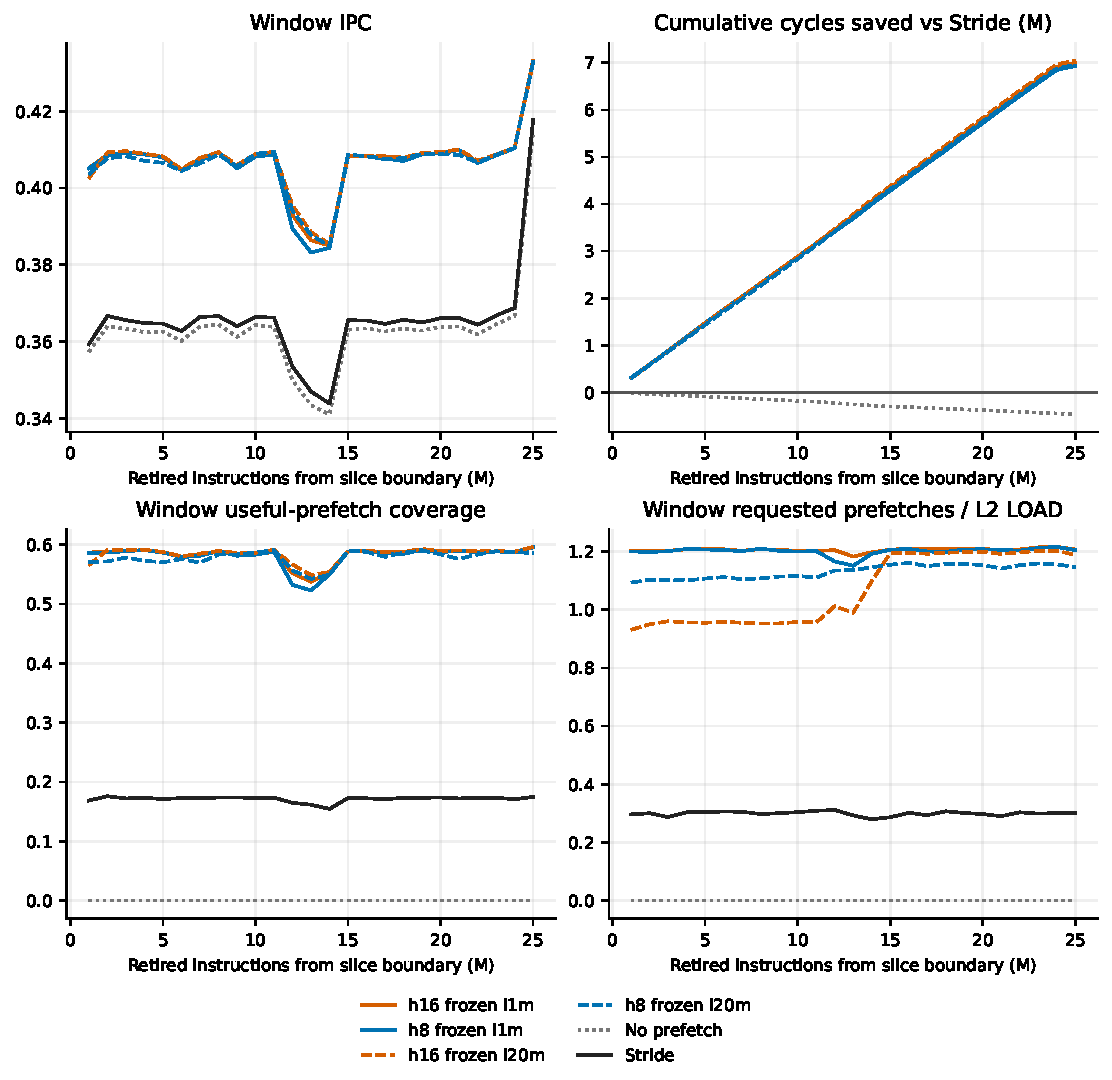
\includegraphics[width=0.98\linewidth]{figures/functional_progress.pdf}\end{center}

These are live fixed-weight runs. Changing window behavior reflects incoming accesses, evolving h/c, cache state and realized timing; it does not indicate parameter learning. The cumulative curve retains all startup costs. The h8 and h16 i1m/i20m curves are separate checkpoints, with solid i1m and dashed i20m traces.

\clearpage\section{Quality and traffic over execution}

\begin{center}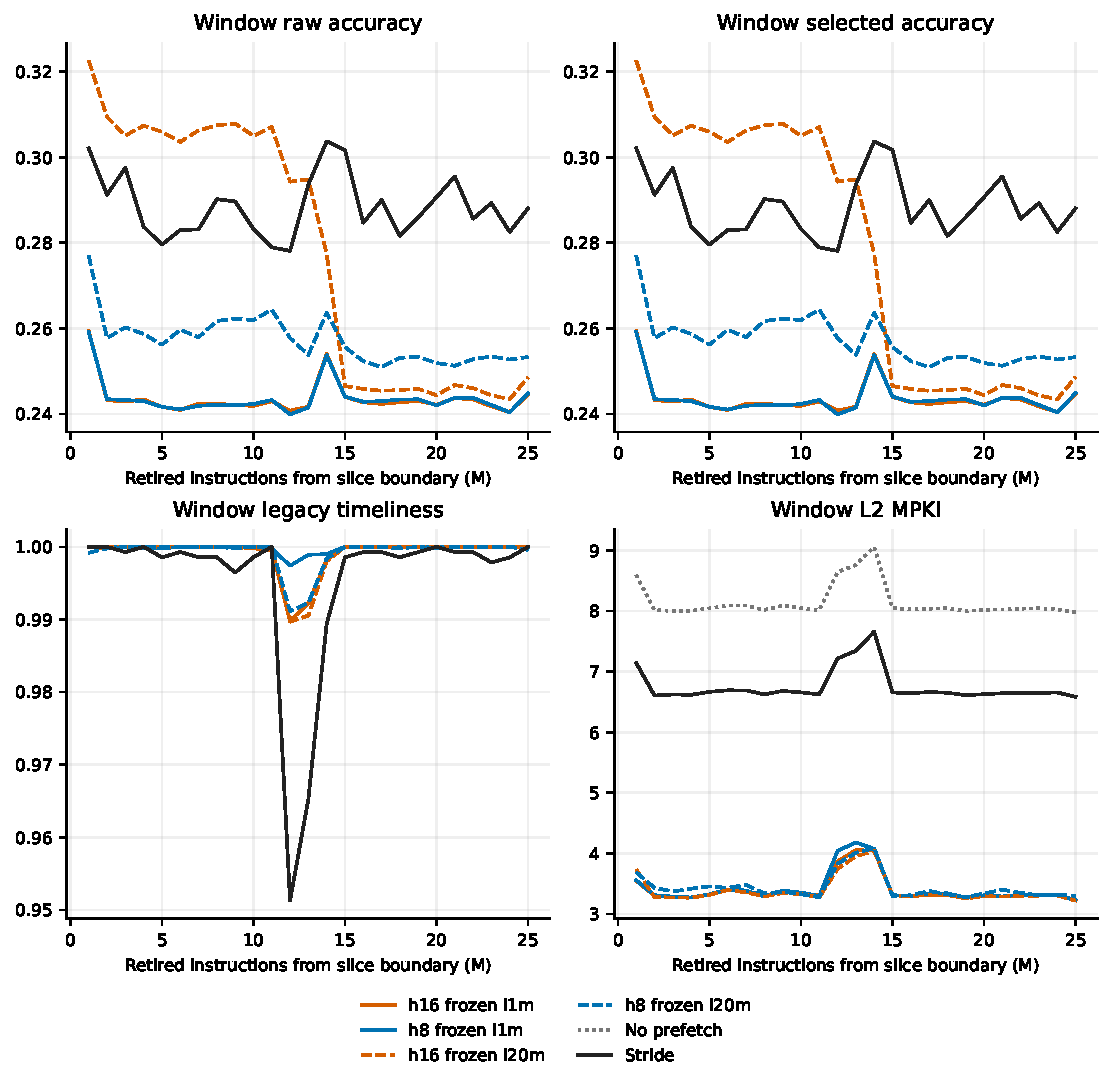
\includegraphics[width=0.98\linewidth]{figures/functional_quality.pdf}\end{center}

A request can cross a window boundary before its first useful demand. These ratios use legacy counter activity within each interval, so a denominator can be zero even when a useful event occurs. NA remains missing, not zero or failure. Separate issue-cohort outcomes retain pending and resident-unused requests as censored. The committed issue-cohort table contains timely, late, unused, redundant and censored counts rather than replacing a legacy metric under the same name.

\clearpage\section{L2 occupancy and turnover}

\begin{center}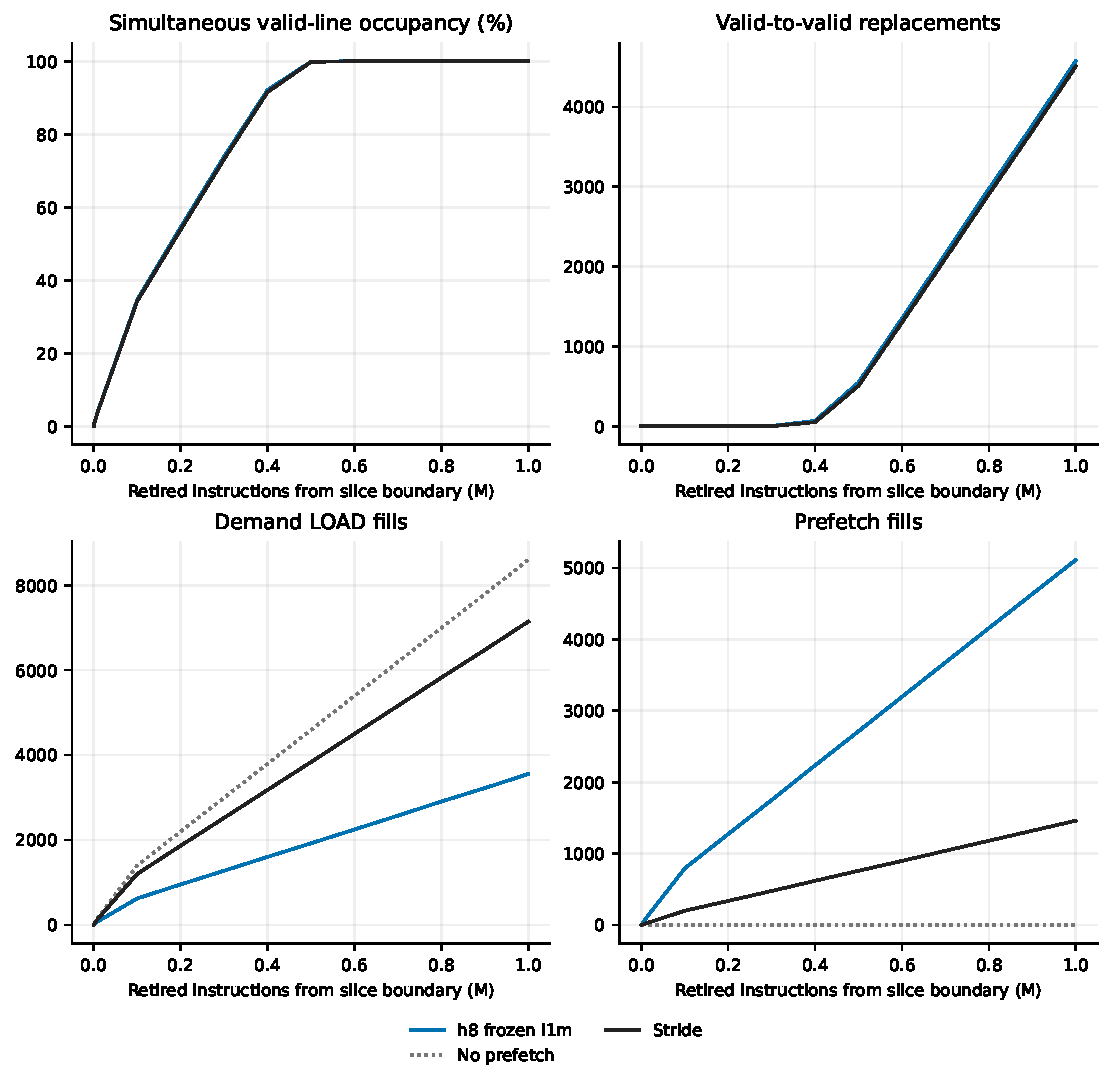
\includegraphics[width=0.98\linewidth]{figures/cache_progress.pdf}\end{center}

The active L2 has 512 sets, 8 ways and 64-byte lines: 4,096 lines or 256 KiB. Occupancy counts simultaneous valid lines, verified against a scan at samples. Invalid-to-valid fill raises occupancy; valid-to-valid replacement does not. The first million instructions show filling alongside ongoing turnover, not a deadline for prefetch usefulness. Fullness does not establish a warmed working set.

\clearpage\subsection{Exact occupancy attainment and fill outcomes}

\begin{center}
\scriptsize
\begin{tabular}{lrrrrrr}
\toprule
Method & 50\% ins. & 90\% ins. & 95\% ins. & 99\% ins. & 100\% ins. & 100\% cycles \\
\midrule
h16 frozen i1m & 177,051 & 388,585 & 417,448 & 460,465 & 536,006 & 1,334,339 \\
h8 frozen i1m & 176,919 & 388,585 & 417,448 & 460,465 & 536,006 & 1,334,484 \\
h8 frozen i1m /64 /MAC0 & 176,919 & 388,585 & 417,448 & 460,465 & 536,006 & 1,334,484 \\
h8 frozen i1m /64 /MAC16 & 179,239 & 391,448 & 419,800 & 461,325 & 536,244 & 1,519,001 \\
h8 frozen i1m /64 /MAC4 & 179,479 & 391,448 & 420,040 & 461,425 & 536,244 & 1,520,031 \\
h16 frozen i20m & 175,639 & 387,882 & 417,242 & 460,385 & 536,006 & 1,351,583 \\
h8 frozen i20m & 177,451 & 389,020 & 418,220 & 460,687 & 536,006 & 1,342,677 \\
No prefetch & 180,391 & 392,060 & 420,440 & 461,565 & 536,244 & 1,520,774 \\
Stride & 180,091 & 391,562 & 420,040 & 461,565 & 536,244 & 1,512,126 \\
\bottomrule
\end{tabular}
\end{center}

\begin{center}
\scriptsize
\begin{tabular}{lrrrrr}
\toprule
Method & LOAD fills & RFO fills & PF fills & WB fills & Replacements \\
\midrule
h16 frozen i1m & 85,022 & 2 & 122,123 & 0 & 203,051 \\
h8 frozen i1m & 85,475 & 2 & 121,310 & 0 & 202,691 \\
h8 frozen i1m /64 /MAC0 & 85,477 & 2 & 121,304 & 0 & 202,687 \\
h8 frozen i1m /64 /MAC16 & 202,455 & 2 & 2,933 & 0 & 201,294 \\
h8 frozen i1m /64 /MAC4 & 203,238 & 2 & 1,607 & 0 & 200,751 \\
h16 frozen i20m & 84,784 & 2 & 123,592 & 0 & 204,282 \\
h8 frozen i20m & 86,101 & 2 & 122,053 & 0 & 204,060 \\
No prefetch & 203,764 & 2 & 0 & 0 & 199,670 \\
Stride & 168,865 & 2 & 35,439 & 0 & 200,210 \\
\bottomrule
\end{tabular}
\end{center}

All listed cold runs reached full occupancy; exact first-attainment instruction/cycle counters are in occupancy\_milestones.csv. LOAD, RFO, prefetch and writeback fills retain distinct meanings. Useful line lifetimes and fill-to-first-demand timing are in resources.csv. Request lifecycle observations are measurement-only and are not neural features.

\begin{center}
\scriptsize
\begin{tabular}{lrrrrrrr}
\toprule
Method & Enqueued & Timely & Late & Unused & Cache red. & Flight red. & Censored \\
\midrule
h16 frozen i1m & 487,444 & 118,744 & 99 & 3,329 & 322,363 & 42,859 & 50 \\
h8 frozen i1m & 485,458 & 118,291 & 25 & 2,974 & 321,748 & 42,375 & 45 \\
h8 frozen i1m /64 /MAC0 & 485,437 & 118,288 & 25 & 2,971 & 321,736 & 42,372 & 45 \\
h8 frozen i1m /64 /MAC16 & 166,466 & 1,310 & 2 & 1,607 & 163,529 & 2 & 16 \\
h8 frozen i1m /64 /MAC4 & 91,858 & 526 & 6 & 1,071 & 90,241 & 4 & 10 \\
h16 frozen i20m & 432,486 & 118,982 & 108 & 4,556 & 264,963 & 43,823 & 54 \\
h8 frozen i20m & 457,373 & 117,666 & 98 & 4,334 & 290,092 & 45,130 & 53 \\
No prefetch & 0 & 0 & 0 & 0 & 0 & 0 & 0 \\
Stride & 121,020 & 34,900 & 168 & 535 & 50,484 & 34,929 & 4 \\
\bottomrule
\end{tabular}
\end{center}

Cohorts use unique enqueue and first-demand lifecycle accounting. They are supplementary and need not equal the legacy useful/late counters. Pending/in-flight and resident-unused outcomes remain censored at the final boundary rather than being assigned failure.

\clearpage\section{Finite-service negative results}

\begin{center}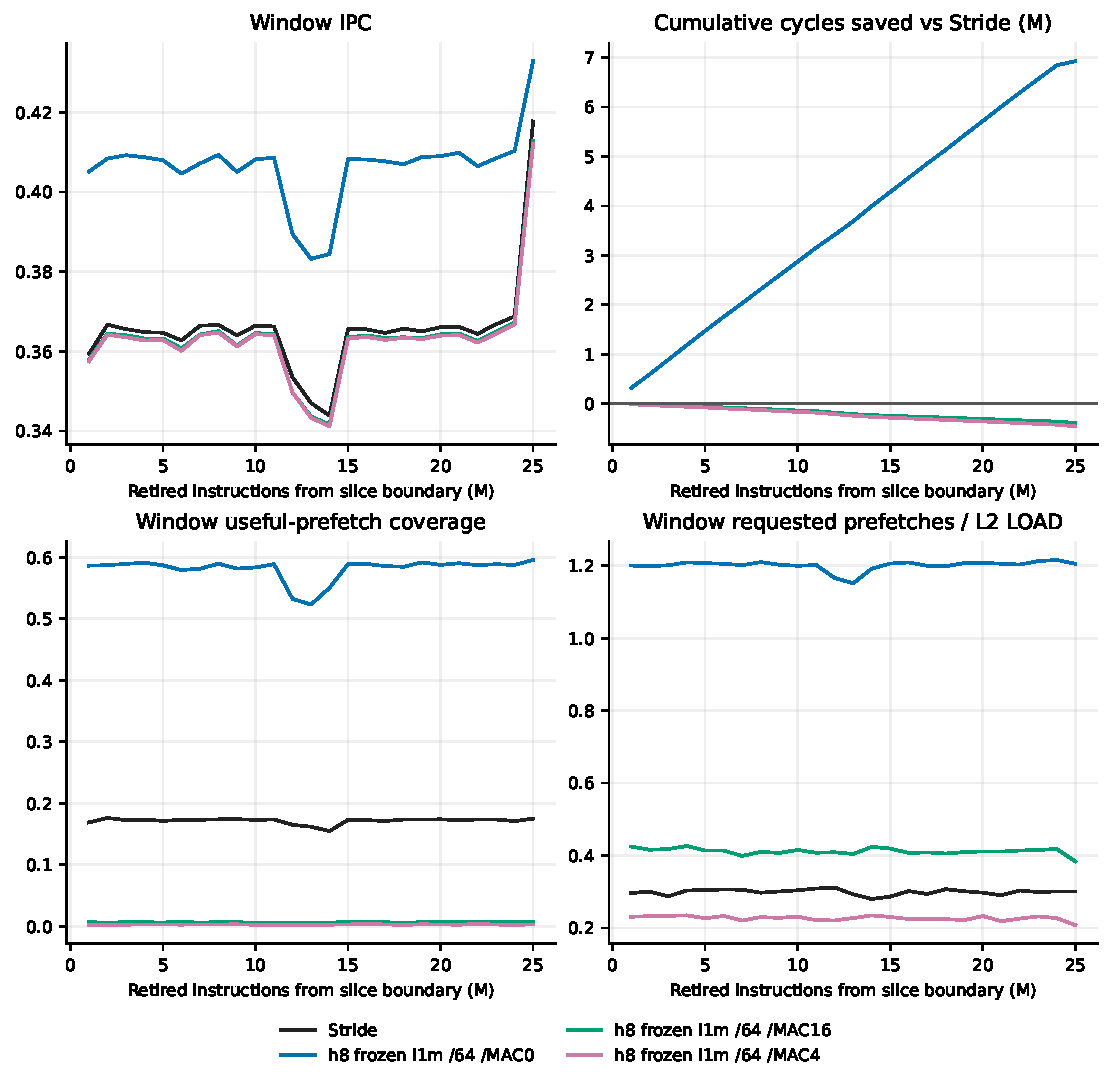
\includegraphics[width=0.98\linewidth]{figures/finite_progress.pdf}\end{center}

The frozen 4/16-MAC cases remain below matched Stride end to end. The same finite table at zero cost isolates the table capacity choice. The timed MAC4/MAC16 cases have zero state evictions, so their losses cannot be attributed to h/c eviction. The finite zero-cost control records 30 evictions.

\clearpage\subsection{Inference work, admission and completion}

\begin{center}
\scriptsize
\begin{tabular}{lrrrrrr}
\toprule
Case & Eligible & Admitted & Completed & Input drops & States peak & Evictions \\
\midrule
h8 frozen i1m /64 /MAC0 & 404,271 & 404,271 & 404,271 & 0 & 64 & 30 \\
h8 frozen i1m /64 /MAC16 & 404,271 & 152,079 & 152,062 & 252,192 & 63 & 0 \\
h8 frozen i1m /64 /MAC4 & 404,271 & 84,108 & 84,091 & 320,163 & 57 & 0 \\
\bottomrule
\end{tabular}
\end{center}

\begin{center}
\scriptsize
\begin{tabular}{lrrrrr}
\toprule
Case & MAC/decision & Nonlinear/decision & Service cycles & Input peak & Output peak \\
\midrule
h8 frozen i1m /64 /MAC0 & 1,825.78 & 78.62 & 0 & 1 & 2 \\
h8 frozen i1m /64 /MAC16 & 1,801.60 & 75.92 & 68,888,246 & 16 & 2 \\
h8 frozen i1m /64 /MAC4 & 1,801.06 & 75.86 & 68,958,580 & 16 & 2 \\
\bottomrule
\end{tabular}
\end{center}

Work averages use actual started decisions and decoded K. Finite service combines inference throughput, queued state dependencies and address arrival delay. Pending decisions at the endpoint remain pending. Queue pressure and redundant issued requests explain why a useful zero-cost algorithm can lose under these modeled resources. This does not demonstrate that every hardware implementation would have the same service cost.

\section{Frozen deployment storage}

\begin{center}
\small
\begin{tabular}{lrr}
\toprule
h8, 64 entries: component & Configured KiB & Observed component peak KiB \\
\midrule
active FP32 weights & 7.453 & 7.453 \\
PC tags, metadata and h/c & 6.000 & 5.344 \\
inference scratch & 1.312 & 1.312 \\
active event metadata & 0.055 & 0.055 \\
decoded delta/address payload & 0.500 & 0.031 \\
input queue & 0.875 & 0.875 \\
output queue & 0.750 & 0.047 \\
\bottomrule
\end{tabular}
\end{center}

The h8 model has 1,908 FP32 parameters: 7,632 bytes (7.453125 KiB). H16 has 5,220 parameters: 20,880 bytes (20.390625 KiB). One state entry reserves 32 bytes for exact-PC tag/metadata and 8H bytes for FP32 h/c. Scratch, active event, decoded output and input/output queues are additional deployment storage. There is no neural shadow teacher, training buffer, gradient, optimizer state, training weight copy or publication buffer in frozen deployment.

\begin{center}
\scriptsize
\begin{tabular}{lrr}
\toprule
Method & Configured total KiB & Sum of observed component peaks KiB \\
\midrule
h16 frozen i1m & NA & 37.078 \\
h8 frozen i1m & NA & 17.578 \\
h8 frozen i1m /64 /MAC0 & 16.945 & 14.953 \\
h8 frozen i1m /64 /MAC16 & 16.945 & 15.680 \\
h8 frozen i1m /64 /MAC4 & 16.945 & 15.117 \\
h16 frozen i20m & NA & 37.078 \\
h8 frozen i20m & NA & 17.578 \\
No prefetch & 0.000 & 0.000 \\
Stride & 2.016 & 2.016 \\
\bottomrule
\end{tabular}
\end{center}

\textbf{Refactored layout versus retained measurements.} The retained scientific runs used a 56-byte active event and a 16-by-56-byte input queue. The frozen-only refactor removes unused event fields, reducing these to 24 bytes and 16-by-24 bytes. Its configured h8/64-entry deployment is therefore 16,808 bytes (16.414 KiB), compared with the original measured layout's 17,352-byte reservation (16.945 KiB): a 544-byte structural reduction. These revised configured bytes are derived from the current packed layout, not retroactively measured allocation peaks. The component-peak and scientific counters above remain those recorded by the original frozen runs.

Unbounded state has no finite configured maximum (NA). Summed component peaks are an envelope, not a simultaneous allocation measurement. Fixed scratch reservations are not allocator measurements. The Stride row includes only its conventional baseline state. Measurement logging and host allocator/RSS overhead are excluded. Dedicated predictor SRAM is compared with the 256 KiB L2 by size; it is not assumed to occupy or pollute L2. These FP32 counts are not quantized deployment measurements.

\clearpage\section{Offline budget and historical frozen compatibility}

Offline i1m used 16,172 decisions, 2,486 positive decisions and 4,875 action atoms, with 12 epochs and 228 optimizer steps. I20m used 325,389 decisions, 52,059 positive decisions and 102,140 action atoms, with 12 epochs and 4,404 optimizer steps. These are offline model-preparation observations. They are not runtime observations or fixed-weight deployment allocations.

The previously reported 1M plateau concerns the offline pretraining budget across the completed prefix sweep. It does not mean a frozen runtime learns after one million observations, nor does similar IPC establish identical action behavior. I1m/i20m retain separate rows and their own traffic measurements. The completed historical live logs establish behavior directly; missing logs would not establish equivalence.

\begin{center}
\scriptsize
\begin{tabular}{llrrrr}
\toprule
Model & Original transport & IPC & Cycles & Coverage & Pressure \\
\midrule
h8 i1m & offline keyed replay & 0.409124 & 61,106,147 & 0.5799 & 0.8776 \\
h8 i1m & frozen live parity & 0.409139 & 61,103,980 & 0.5800 & 0.9519 \\
h8 i20m & offline keyed replay & 0.409244 & 61,088,223 & 0.5757 & 1.0162 \\
h8 i20m & frozen live parity & 0.409254 & 61,086,777 & 0.5757 & 1.1259 \\
h16 i1m & offline keyed replay & 0.409730 & 61,015,850 & 0.5832 & 1.0821 \\
h16 i1m & frozen live parity & 0.409738 & 61,014,571 & 0.5832 & 1.2089 \\
h16 i20m & offline keyed replay & 0.409938 & 60,984,797 & 0.5845 & 0.9744 \\
h16 i20m & frozen live parity & 0.409946 & 60,983,624 & 0.5846 & 1.0726 \\
\bottomrule
\end{tabular}
\end{center}

\begin{center}
\scriptsize
\begin{tabular}{lrrr}
\toprule
Preserved compatibility run & Original parser fields exact & Instructions & Cycles \\
\midrule
h16 frozen i1m & 30/30 & 25,000,003 & 61,014,571 \\
h8 frozen i1m & 30/30 & 25,000,003 & 61,103,980 \\
h16 frozen i20m & 30/30 & 25,000,003 & 60,983,624 \\
h8 frozen i20m & 30/30 & 25,000,003 & 61,086,777 \\
\bottomrule
\end{tabular}
\end{center}

Each of the four historical frozen checks matches all 30 original parser fields, 120/120 in total. These are preserved measurements from the predecessor source, with no claim that this refactor newly executed the full historical protocol. The original no-prefetch historical reference has 203,131 measured L2 LOAD misses; it is used only for historical end metrics, never cold windows. Historical warm-cache IPC is not compared against cold-cache IPC as a performance gain.

\section{Interpretation and limits}

On this one held-out trace slice, offline-trained frozen inference provides useful zero-cost live prefetching with dynamic recurrent state. H8 already captures most of the measured i1m/i20m IPC behavior at lower weight cost than h16. The finite 4/16-MAC results expose queueing and lateness costs that erase that benefit under the stated architectural assumptions. They are retained as negative results. One trace and one pretraining seed do not establish generalization across workloads or statistical equivalence.

The branch's active entry point is run.py; design.md defines the fixed-weight conditions, and command.md records build/test/run/status/resume/report commands and report compilation. Compact raw counters and figure inputs are committed. SPEC traces, checkpoints and full raw logs remain in their existing private trees. All plotted scientific rows are actual frozen or conventional baseline measurements; weight-changing scientific rows are excluded rather than renamed. The raw reference paths continue to identify their original measurements.

\end{document}
